
\usetikzlibrary{positioning, arrows.meta}
\section{ML-Pipeline}
This section covers the pipeline for training the phishing detection model as well as the different tools used. Furthermore it explains some of the shortcomings of the pipeline.

\subsection{Pipeline}
The pipeline is managed by DVC and consists of following three stages: preprocessing, training, and testing. The pipeline was designed such that after each of these stages intermediate output files could be created which can serve as checkpoints for the next stage. An overview of the pipeline can be found in \autoref{fig:mlpipeline}.


\subsection{Tools}
The project relies on DVC for both pipeline management and data version control. This allows for great reproducibility as well as efficient data management. Furthermore google drive was used for remote storage. One google drive folder manages all the DVC artifacts, while a seperate google drive folder contains the models and related files specifically for deployment. These files are downloaded during runtime of model-service. This allows for swapping of the models without creating a new image.

\subsection{Shortcomings}
A major shortcoming of the pipeline is that it is only partially automated as some artifacts still need to be manually uploaded to the separate drive folder that was created specifically for deployment. This can be very error prone as this can not only introduce human error but it also means that the manually uploaded version for deployment is not versioned. This makes it not immediately clear which version of the model is currently deployed.



\begin{figure}[h!]
    \centering
    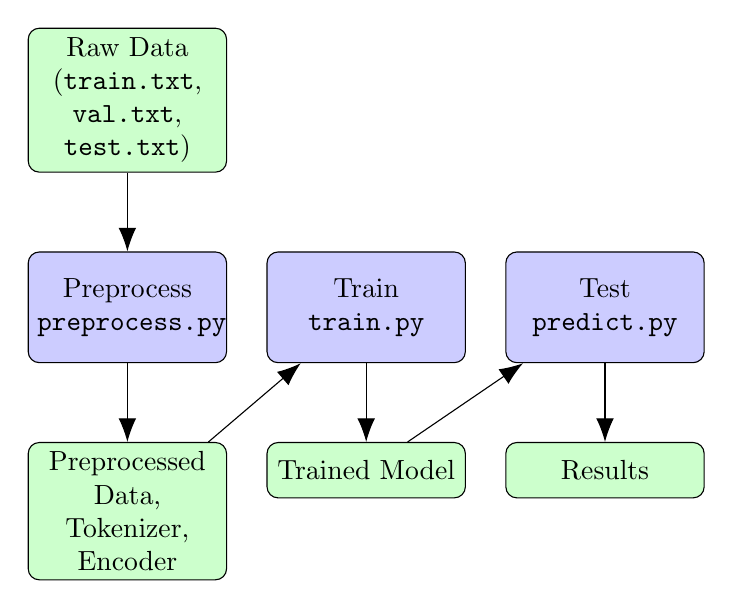
\begin{tikzpicture}[
        node distance=1cm and 0.5cm,
        stage/.style={rectangle, draw, fill=blue!20, text width=6.5em, text centered, minimum height=4em, rounded corners},
        artifact/.style={rectangle, draw, fill=green!20, text width=6.5em, text centered, minimum height=2em, rounded corners},
        arrow/.style={draw, -{Latex[length=3mm]}}
    ]
    
    % Nodes
    \node (preprocess) [stage] {Preprocess\\ \texttt{preprocess.py}};
    \node (train) [stage, right=of preprocess] {Train\\ \texttt{train.py}};
    \node (test) [stage, right=of train] {Test\\ \texttt{predict.py}};
    
    \node (raw_data) [artifact, above=of preprocess] {Raw Data\\ (\texttt{train.txt}, \texttt{val.txt}, \texttt{test.txt})};
    \node (processed_data) [artifact, below=of preprocess] {Preprocessed Data, \\ Tokenizer, \\ Encoder};
    \node (trained_model) [artifact, below=of train] {Trained Model};
    \node (results) [artifact, below=of test] {Results};

    % Arrows
    \draw [arrow] (raw_data) -- (preprocess);
    \draw [arrow] (preprocess) -- (processed_data);
    \draw [arrow] (processed_data) -- (train);
    \draw [arrow] (train) -- (trained_model);
    \draw [arrow] (trained_model) -- (test);
    \draw [arrow] (test) -- (results);
    
    \end{tikzpicture}
    \caption{ML Pipeline}
    \label{fig:mlpipeline}
\end{figure}